%------------------------------------------------
\section{All Pairs Shortest Paths (APSP)} 

\subsection{Idee} 

\begin{frame}
\frametitle{APSP - All Pairs Shortest Paths}
\begin{block}{Problemstellung}
Man hat einen Graphen gegeben, der gewichtet ist. Nun möchte man den kürzesten Pfad zwischen allen Knoten i zu allen Knoten j herausfinden.
\end{block}
\end{frame}

%------------------------------------------------

\begin{frame}
\frametitle{APSP - Erster Ansatz}
\begin{block}{Lösungsansatz}
Man verwendet den bereits bekannten SSSP-Algorithmus, und führe diesen nach bedarf aus, d.h. in diesem Fall $|V|$-mal.
\end{block}

\begin{block}{Laufzeit}
$|V| \cdot O (|E| + |V| \cdot log(|V|))$\\$
= |V| \cdot O (|V|^2 + |V| \cdot log(|V|))$\\$ fehler
= |V| \cdot O ((|V|^2) \cdot log(|V|)) $\\$ fehler 
= O ((|V|^3) \cdot log(|V|))$\\
$\implies$ geht es einfacher in etwa der selben Zeit?
\end{block}
\end{frame}

%------------------------------------------------

\begin{frame}
\frametitle{APSP - Zweiter Ansatz}
\begin{block}{Lösungsansatz}
Wir wissen: jeder Pfad zwischen zwei Knoten ist entweder bereits der kürzeste, oder es gibt einen Kürzeren Pfad als zwei Verknüpfung anderer Pfade über mindestens einen dritten Knoten.
\end{block}

\begin{block}{Genauer}
Systematisch in einer Adjazenzmatrix A:
Nehme für jeden Pfad $A[i][j] = \min\left(A[i][j], A[i][k] + A[i][k]\right)$, d.h. entweder der Pfad ist bereits minimal, oder ein Pfad über Knoten k ist kürzer und wird als neues Minimum übernommen.
Wenn man nun richtig iteriert, erhält man alle minimalen Pfade.
\end{block}
\end{frame}

%------------------------------------------------

\subsection{Code}

\begin{frame}[fragile] % Need to use the fragile option when verbatim is used in the slide
\frametitle{Code}

\begin{lstlisting}
for (int k = 0; k < V; k++)
    for (int i = 0; i < V; i++)
        for (int j = 0; j < V; j++)
            A[i][j] = min(
              A[i][j],
              A[i][k] + A[k][j]
            );
\end{lstlisting}

~\\$\implies$ der Aufwand liegt in $O(|V|^3)$

\end{frame}

%------------------------------------------------

\begin{frame}
\frametitle{Beispiel - Urzustand}

\includegraphics[width=\linewidth]{floyd_warshall_graphs/graph1.JPG}

\end{frame}

%------------------------------------------------

\begin{frame}
\frametitle{Beispiel - Über Knoten A}

\includegraphics[width=\linewidth]{floyd_warshall_graphs/graph2.JPG}

\end{frame}

%------------------------------------------------

\begin{frame}
\frametitle{Beispiel - Über Knoten B}

\includegraphics[width=\linewidth]{floyd_warshall_graphs/graph3.JPG}

\end{frame}

%------------------------------------------------

\begin{frame}
\frametitle{Beispiel - Über Knoten C}

\includegraphics[width=\linewidth]{floyd_warshall_graphs/graph4.JPG}

\end{frame}

%------------------------------------------------

\begin{frame}
\frametitle{Beispiel - Über Knoten D (1)}

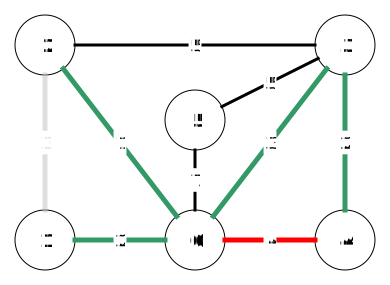
\includegraphics[width=\linewidth]{floyd_warshall_graphs/graph5.JPG}

\end{frame}

%------------------------------------------------

\begin{frame}
\frametitle{Beispiel - Über Knoten D (2)}

\includegraphics[width=\linewidth]{floyd_warshall_graphs/graph6.JPG}

\end{frame}

%------------------------------------------------

\begin{frame}
\frametitle{Beispiel - Über Knoten D (3)}

\includegraphics[width=\linewidth]{floyd_warshall_graphs/graph7.JPG}

\end{frame}

%------------------------------------------------

\begin{frame}
\frametitle{Beispiel - Über Knoten D (4)}

\includegraphics[width=\linewidth]{floyd_warshall_graphs/graph8.JPG}

\end{frame}

%------------------------------------------------

\begin{frame}
\frametitle{Beispiel - Über Knoten D (5)}

\includegraphics[width=\linewidth]{floyd_warshall_graphs/graph9.JPG}

\end{frame}

%------------------------------------------------

\begin{frame}
\frametitle{Beispiel - Über Knoten D (6)}

\includegraphics[width=\linewidth]{floyd_warshall_graphs/graph10.JPG}

\end{frame}

%------------------------------------------------

\begin{frame}
\frametitle{Weitere Anwendungen}
\begin{itemize}

\item Auch für SSSP - Probleme anwendbar (wenn $\vert V \vert < 400$)
\item Detektion von negativen oder günstigsten Zyklen möglich $\implies$ ein negativer Zyklus existiert genau dann, wenn ein Diagonaleintrag negativ ist
\item Finden des Durchmessers eines Graphen (der längste der kürzesten Pfade)
\item Minimax, Maximin
\end{itemize}
\end{frame}

%------------------------------------------------

\subsection{Beurteilung} 

\begin{frame}
\frametitle{Beurteilung}
\begin{itemize}

\item[+] Asymptotische Komplexität $\in O(|V|^3)$  und mit Speicher $\in O(|V|^2)$
\item[+] Sehr leicht zu implementieren (Vierzeiler)
\item[+] Für andere Probleme günstig anzuwenden, wenn $|V|< 400$
\item[-- --] Für andere Probleme \textbf{nur} günstig anzuwenden, wenn $|V|< 400$
\end{itemize}

$\implies$ Gut für das ursprüngliche Problem\\
$\implies$ Auch nützlich für andere Probleme, solange $|V| < 400$
\end{frame}

%------------------------------------------------

\section{Zusammenfassung}

\begin{frame}
\frametitle{Zusammenfassung}
\small{\begin{table}
\begin{tabular}{l l l l}
\toprule
\textbf{Kriterium} & \textbf{Dijkstra} & \textbf{Bellman Ford} &\textbf{Floyd Warshall}\\
\midrule
Laufzeit & $O(V+E)\log(V)$ & $O(V \cdot E)$ & $O(V^3)$ \\
Max. Größe  & $V,E \leq 300K$ & $V,E \leq 10M$ & $V \leq 400$ \\
Ungewichtet & Ok & Schlecht & I.A. Schlecht \\
Gewichtet & Bestes & Ok & I.A. Schlecht \\
Neg. Gewichte & Ok & Ok & I.A. Schlecht \\
Neg. Zyklen & Nein & Aufspürbar & Aufspürbar \\
Kleine Graphen & Overkill & Overkill & Bestes \\
\bottomrule
\end{tabular}
\caption{Übersicht}
\end{table}}
Anmerkung: Lese $V$ als $|V|$ und $E$ als $|E|$
\end{frame}

%------------------------------------------------